% Created 2021-04-12 Mon 12:07
% Intended LaTeX compiler: pdflatex
\documentclass[9pt, b5paper]{article}
\usepackage[UTF8]{ctex}
\usepackage{fontspec}
\usepackage{graphicx}
\usepackage{xcolor}
\usepackage{multirow}
\usepackage{multicol}
\usepackage{float}
\usepackage{textcomp}
\usepackage{geometry}
\geometry{left=1.2cm,right=1.2cm,top=1.5cm,bottom=1.2cm}
\usepackage{algorithm}
\usepackage{algorithmic}
\usepackage{latexsym}
\usepackage{natbib}
\usepackage{listings}
\usepackage{minted}
\usepackage[xetex,colorlinks=true,CJKbookmarks=true,linkcolor=blue,urlcolor=blue,menucolor=blue]{hyperref}
\author{Deepwaterooo Wang}
\date{\today}
\title{成长的故事——我和舅舅}
\hypersetup{
 pdfauthor={Deepwaterooo Wang},
 pdftitle={成长的故事——我和舅舅},
 pdfkeywords={},
 pdfsubject={},
 pdfcreator={Emacs 27.1 (Org mode 9.3)}, 
 pdflang={English}}
\begin{document}

\maketitle
\tableofcontents


\section{遥忆2011年3月三大locate到职场的第一份被逼当性奴的工作}
\label{sec:org77b90fb}

\begin{center}

\includegraphics[width=.9\linewidth]{./pic/backups_plans_p1p143-1.png.png}
\end{center}

这篇主要借后来2012年10月对统计专业2011年3月第一份三大locate到职场并想要逼良为娼的工作作一个回忆和分析,供广大女留学生、广大女性朋友们、社会大家擦亮眼睛、火眼金睛地借鉴。

我的记忆不是很好,距离2011年事件真正过去已经很多年了,很多细节我想不想来。我仅凭自己先前的传记中有限的文字记载、和我能够回忆起的人事物来作合理假设推测推理,请读者明鉴。

\begin{center}
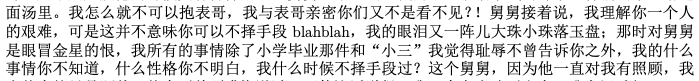
\includegraphics[width=.9\linewidth]{./pic/backups_plans_20210412_103658.png}
\end{center}

首先,我们看到,在2011年2月份我第一次主动回表哥家想要向表哥表白时,舅舅就已经在那次我即将离开时,对我提出严厉批评:舅舅批评我、说我“不择手段”?

\begin{center}
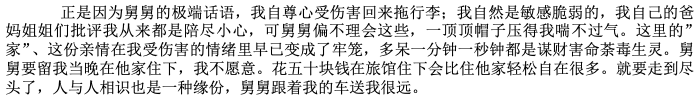
\includegraphics[width=.9\linewidth]{./pic/backups_plans_20210412_110028.png}
\end{center}
舅舅批评我的当时、当下,舅舅的话太重太痛了,我是无论如何、当时的自己也接受不了的!

那么我成长的历史上,我所受过的批评,我都能很好地接受吗?

\begin{center}
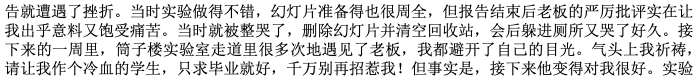
\includegraphics[width=.9\linewidth]{./pic/backups_plans_20210412_110225.png}
\end{center}

国内硕士时的老板对自己的一次严厉的批评:我痛了很久、痛了一个星期,都不想要再理会自己的导师,只想作个冷血的学生,只求能够顺利毕业就好!

\begin{center}
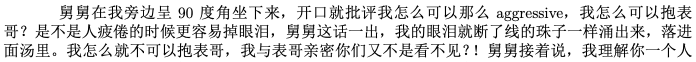
\includegraphics[width=.9\linewidth]{./pic/backups_plans_20210412_110604.png}
\end{center}

\begin{center}
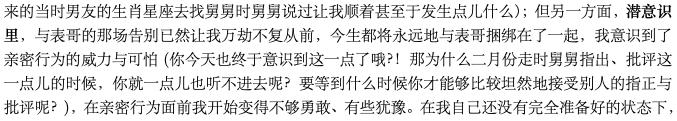
\includegraphics[width=.9\linewidth]{./pic/backups_plans_20210412_110513.png}
\end{center}

也有正面的例子。在舅舅指出相当于是男女有别、我是不可以随便碰表哥、我是不可以随便碰到、身体肢体接触到其它人的这份教导里,至少有一次机会让我潜意识里意识到:舅舅的教导是对的,有些事情我不敢随便、也不应该随便!比如,我是不可以随便再碰表哥的!

及至今年3月、阔别六年再见到表哥,我看表哥永远看不够、且情不自禁地抓了表哥的手又一次地碰了表哥,实在是情不自禁,这是后话。 

在我的印象里,舅舅是个观察力敏锐的社会观察家,是舅舅先知先觉地知道了什么?是舅舅在浏览三大网页的时候,已然注意到三大炒作的苗头不太对?那里的我对于三大的炒作基本完全不知道是怎么回事,就当这是一种可能性吧。

还是,舅舅是在预测,他是预测在一个女孩子的职场工作中她可能会碰到的危险情况,继而以这种过于强硬的教导来训戒我?

\begin{center}
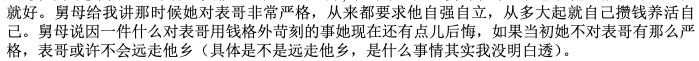
\includegraphics[width=.9\linewidth]{./pic/backups_plans_20210412_112222.png}
\end{center}

而这,也与先前舅母给我提到我的表哥,他们作为父母对于我表哥的严格要求是相一致的。

如果舅舅能够把我这个远亲的侄女同他自己的亲生儿子、天才儿子我的表哥一样看待和要求,我心里对舅舅是万分感激的:我感激舅舅对我的教导,也深深感激舅舅能够把我同自己的天才表哥同等、平起平坐地看待!
\begin{center}
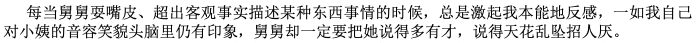
\includegraphics[width=.9\linewidth]{./pic/backups_plans_20210412_114832.png}
\end{center}

早年与舅舅聊天聊及我仍有印象的哑巴小姨,我的舅舅口吐莲花般地向我描绘小姨是怎样一个冰雪聪明的女孩子,但只是因为小时候生病、没有医疗条件没能够得到及时的救治延误了时机,小姨后来耳朵聋了听不见声音、不会说话。但她仍然是那样一个极其聪明的女孩。当时对舅舅的家庭有成见的我,表达的都是对舅舅的成见,却不知,反过来想,我也同哑巴小姨一样、没有很好的求学、受教育机会。如果我能够好好投胎投胎到舅舅家里,今天的我应该绝不是现在的这个样子吧!可是舅舅对人性的深深了悟,让我坚信,一如舅舅,表哥也不会嫌弃我笨或是傻,他们待我有着发自心底的深深同情与尊重,让我深为动容,感泣不已!

舅舅能够做到这一点,让我极为动容,实在不是凡夫俗子能够达到的境界。

\begin{center}
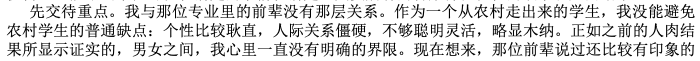
\includegraphics[width=.9\linewidth]{./pic/backups_plans_20210412_104246.png}
\end{center}

男女之间,我心里一直没有明确的界限。

在国内硕士期间硕二进实验室的时候,我甚至一度几乎要掉进喜欢一个已婚师兄的坑里,虽然后来是掉进了硕士导师那一边。但我的成长过程中,没有人教导过我些。而自己个人成长的经历、因为那些年痛苦迷失的经历等,常年呆在校园、很是单纯的自己,也没能自己学会这门功课。

\begin{center}
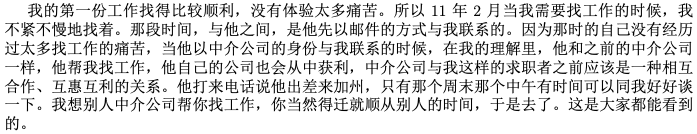
\includegraphics[width=.9\linewidth]{./pic/backups_plans_20210412_104359.png}
\end{center}

\begin{center}
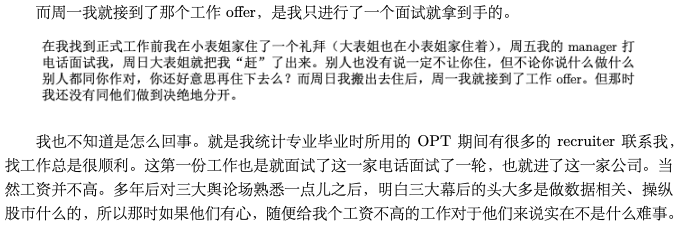
\includegraphics[width=.9\linewidth]{./pic/backups_plans_20210412_113237.png}
\end{center}

\begin{center}
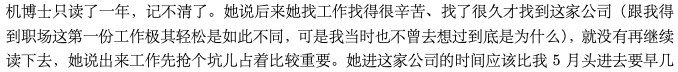
\includegraphics[width=.9\linewidth]{./pic/backups_plans_20210412_113317.png}
\end{center}

我的第一份工作真的是找得极其的轻松(与那时成名告诉我的她找她那职场第一份工作找了很久形成截然不同的对比),因为我的统计专业是落在三大的势力范畴:那时逛三大中文就常年被三大洗脑说,三大背后三个大佬好像是拜过把子的兄弟,都是搞数据相关、搞股票经济什么的。早年舅舅想要我转accounting可以申办H1B的会计专业相关的三大中常常出现在的四大公司,应该都是三大的势力范畴。

\begin{center}
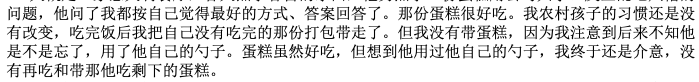
\includegraphics[width=.9\linewidth]{./pic/backups_plans_20210412_104506.png}
\end{center}

他用自已的勺子吃过的蛋糕,我当然是会介意的!

\begin{center}
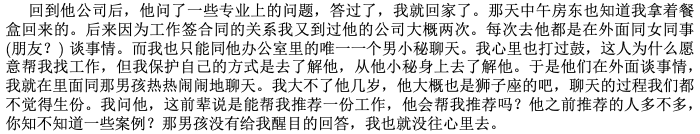
\includegraphics[width=.9\linewidth]{./pic/backups_plans_20210412_104626.png}
\end{center}

人之常情。换作是你,会作出类似的反应,来想要了解更多的相关信息吗?

\begin{center}
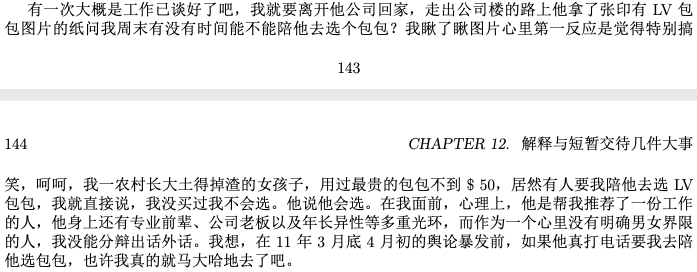
\includegraphics[width=.9\linewidth]{./pic/backups_plans_20210412_104740.png}
\end{center}

\begin{center}
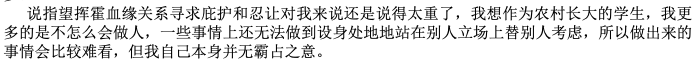
\includegraphics[width=.9\linewidth]{./pic/backups_plans_20210412_114004.png}
\end{center}

\begin{center}
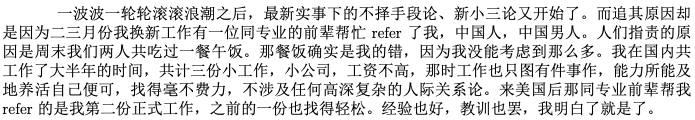
\includegraphics[width=.9\linewidth]{./pic/backups_plans_20210412_114144.png}
\end{center}

这里就有些傻傻的了。可是那些个职场工作早年岁月里的自己,真是常年带点儿人际关系中傻傻分不清楚的感觉!

\begin{center}
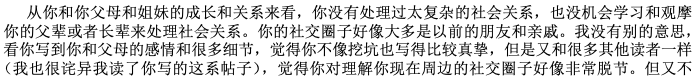
\includegraphics[width=.9\linewidth]{./pic/backups_plans_20210412_114502.png}
\end{center}

有一个网友后来指出来过的我的人际关系的简单,也是一种间接的证明。 

\begin{center}
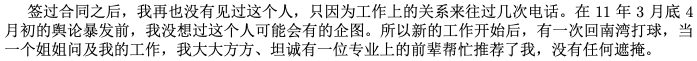
\includegraphics[width=.9\linewidth]{./pic/backups_plans_20210412_104824.png}
\end{center}

与2017年我的专业职场工作,他们会站出来逼相比,11年3月的这份工作是不需要逼的,为什么呢?

四月份的声音说,三大这么多年的紧相与炒作,便宜了中介那个胆大的,说得似乎三大与那份工作的中介没有关系。

但是借着当时充当着我的朋友的成名的联接来看:

她的存在至少是三大的一个托儿的存在

\begin{center}
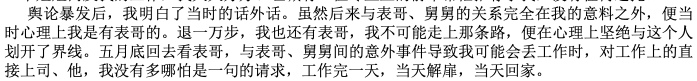
\includegraphics[width=.9\linewidth]{./pic/backups_plans_20210412_104930.png}
\end{center}

四月,当他们舆论的炒作已经把我炒作得面目皆非的时候,我跑回表哥家去找我亲爱的表哥了

那个,这个姑娘,心之所属,是非常清楚的

\begin{center}
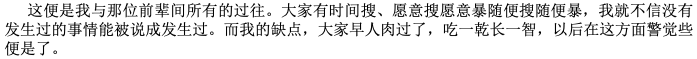
\includegraphics[width=.9\linewidth]{./pic/backups_plans_20210412_104959.png}
\end{center}

五月底的长假,我又早早地与工作中的老板请好假,直接想要加表哥家,三大还有任何可以逼的必要吗?

这份工作的结束,是第一份职场三大逼良为娼,被他们逼着去当职场性奴的第一次、是序幕,却永远不是最后一次!

\textbf{备注:}

现在这篇也写不完了,晚点儿下午五点钟左右再提交一次,把这篇补完,也再提交一篇炒作网红过程记。

\section{三大炒作网红、逼良为娼洗脑记(3):三大自家炒作出的网红是否情商在线、情商上线?}
\label{sec:org0d068ae}

亲爱的读者,由于构篇的原因,前面的内容我没能有条理地组织好。这篇会作必要的补充与连接。

2010年10月,当我说了一句极其幼稚、极其单纯的话,但被一个三大的托儿陷害在其隐藏在正常文字里黄话荤话上下文的隐喻被当作极其放荡的女人发动舆论、进行人肉炒作成他们三大自家的网红。

这个投奔于三大、献忠于三大的他们的托儿,后来拿到三大的回扣这是后话。后来2010、2011年与表哥真正相恋后,再没有与他的任何联系;2015年计算机硕士毕业后我回到加州,他还想微信加我与我联系,当年那么单纯的我被他极端陷害、拖入到三大中文网站的炒作中,我心里始终不平,便果断否绝了他的加载联系人申请,永久与他断联了。这是后话。 

那么,他们,发动舆论进行人肉的导火索点燃之后,三大中文网站炒作一个现实生活中平民百姓家的女孩儿、炒作成他们三大网红的方法是怎样的呢?

同样,根据被盯、被逼当事人反应的不同,在我,仍然是分为了两个不同阶段的操作。

第一个阶段,前期炒作阶段,顺承他们先前三大网站内部人肉我的做法,如同先前提到的三大对我实行实时监听,炒作过程中努力想要与我培养出一种同理心与共情。

从三大盯上我、对我发动炒作,三大对我从来都是实时监听的。

因为我日常生活中的事,会被三大炒作出来,会在当天或是第二天三大首页的网文中有回应(同理心的、感同身受的或是共情的)。

什么样儿的回应呢?比如2012年秋季学期有一天早上我生理期间腹痛,清晨五点钟左右痛醒后就一直痛,我以为自己想上厕所坐马桶,但到了洗手间我又只想躺下;等我躺下,身体还是不舒服,痛得只能躺在床上禁不住连连呻吟,可我还是想去坐马桶,如此反反复复来回了折腾了两三个小时,直到后来实在是痛得、累得不行了,又倒头睡着了一两个小时,后来那天白天上午、身体会有大的血块排出。

那么当天傍晚三大的首页上就出现了(他们的首页是每天傍晚都会更新一次的)相应的回应,说学生时大家都不容易,生病了也舍不得花钱去看医生等能够引起你共情、展现他们想要与你建立一种感情纽带一样的网络回文时常在出现在那几年早年(他们会极尽所能地把他们炒作出的网红打造成世外仙人般的存在一样的清誉、纯净的舆论、三大网红名誉封锁,不允许有任何声音杂音损害这样一个世外天仙般的网红的存在,极力维护打理她的名声。这也是一种舆论与强加的盛名之下被炒作网红的人生封锁)被三大监听的日子。后来2014年春天我从系里拿到TA奖学金,这里面三大也贡献了一点儿力量,这是后话。 

第二个阶段,被盯被炒作当事人被逼疯了自己站出来说话、澄清时的必要操作。 

这里先提一下,10年10月三大已然发动对我的全网人肉、面向社会大众的人肉,为什么到11年11月份我才真正站出来写、写自己的《成长的故事》自传呢?

我们再来回顾一下当年我的情商状态与史实。 

从前面《三大炒作网红、逼良为娼洗脑记(1): 发动人肉、对被盯女性发 动网络炒作并启动对其人生的封锁》里我们已经可以看到,10年10月我被三大的托儿导火索点燃他们发动人肉舆论炒作,当年我的情商是完全跟不上的状态。 

在接下来10年12月与表哥的相处相爱、我在遭遇爱情后想要作世俗社会里垂死的挣扎、本能地想要逃跑的时候,我所有的反应、与当时所谓的朋友(职场上想跟我玩儿成名、以及生活中南湾打球、打羽毛球的朋友)就与表哥关系、对舅舅的不够信任等所说过的话、发表过的过激言论更多的都是出于保护自己的本能,并没有与三大的真正交集。真正的第一次冲突交锋出现在12年春天当我逛过一遍国内校友录、表哥与我经营多年、而我心底始终把表哥视作终生归属的爱情被三大炒作打成稀烂的时候,我急了,跑回去看家里的情况,与舅舅有了一场承上启下、上下各述十年的对话,前面已经交待过。

这里也顺便提一下,当时打球的朋友是否是他们三在的托儿,我不确定,但极有可能都是,因为他们的确切时间点的准时出现,“rebuilding together”,没有三大对我的实时监听、不是三大的托儿是无法那般精确定位地出现在同一时间、同一地点的。 

那么10年10月我被三大的托儿导火索点燃他们发动人肉舆论炒作,而我一直默然不动,又是什么原因迫使我在11年11月最终站出来写自传的呢?

还记得前一篇里我灵魂发问吗:三大中文网站为什么会本能地认定表哥应该是作我男朋友的最佳人选?

我以为那时候三大认定与不认定的两种可能性及推理是:

如果三大一定本能地认定表哥是作我男朋友最佳人选,那么就一定与06年我来美国留学时便同期出现在加州硅谷职场的亲朋圈大表姐王夏华的存在与她在南湾的职场经历(甚至于小表姐王秋勤的过往与此都有关系)有必然关系。这一两个表姐的过往经历,合理猜测、合理推测,能够帮助三大界定表哥与我的恋爱必定是假的、是一场戏、一场表哥假定是我男朋友扮演我男朋友角实、实则舅舅把我当作了人质贡献给他们三大、供他们三大对我进行炒作、继而封锁十年人生、将来被逼良为娼的戏!所以三大会如此认定,如果他们当时真的如此认定的话。

而如果当时三大不曾真正认定,那么他们会拖、他们会采取试探办法去试探表哥与舅舅的立场。

那么自10年12月、表哥或是舅舅已经表达过的立场、不管当时的我是否惊觉、警觉,有哪些呢?我们来列举一下。  

\textbf{图、图、图、截图}

11年2月我回去前,在与舅舅聊天的电话里,舅舅说表哥将来不要小孩都可以!这是与三大炒作出来的自家网红将来被逼作职场性奴、将被逼并不给予生育机会是相契合的;

同期电话里,舅舅骂我性格不好、嫁不出去,潜藏一辈子可能也嫁不了人,同样逼合三大网红、将来被逼作职场性奴、不会有正常婚姻相契合;

11年2月里,我回到表哥家同表哥表白,表哥打发我的第一句话“我十年之内都不会结婚”同样给予了三大中文媒体一剂定心丸。

回去舅舅教育我的立场,舅舅指望两个表姐养老的话,都契合三大立场,因为舅舅没有指望我为他养老,并不拿我真正当作他们家的儿媳妇!舅舅态度鲜明、只批评我的立场同样界定:我只是他们换作将来舅舅的亲侄女王夏华职场生存的筹码,舅舅并不体会、顾及我的立场与感受,我只是泼出去的水、舅舅扔出去的筹码,我的立场与感受,在舅舅及其家人,无关紧要!

同期舅舅表达,只需要把表哥家当作我困顿时、有困难难受时回家修身养性的修心场所,与表哥无丝毫牵连、更与表哥的幸福无关!

11年4月回去与表哥万垂吊俱静、温情无限的今晚也不曾发生过点儿什么,与舅舅两年前埋线(09年春天当我抱着所有打印出来的当时男朋友的生肖属相星座去找舅舅时,舅舅讲话顺应他、不要push的九年之后终成眷属的故事)不符、三大想要炒作的千里迢迢回去只为发生一夜情的界定不符,但并不影响三大对我的炒作与后续封锁。

回到加州后,表哥的邮件态度鲜明地表明,表哥把我当妹妹,批评我私闯表哥的房间!

那么我们可以看到接下来11年5月底我的回表哥家舅舅电话里也同样表明立场:舅舅不欢迎我到舅舅家!

及至月底直接丢掉了工作(本质原因是职场上我的无知无觉、不服管不服他们逼良为娼的逼迫),三大仍然想要采取试探办法去试探表哥与舅舅的立场。

那么我们再来细看一下他们试探的方法与结果是什么呢?

朋友怂勇我与表哥结婚,结婚了就什么问题就解决了。呵呵呵,这傻问题正契合我当时傻傻的头脑与情商,于是我给表哥写邮件了问及表哥的态度,我收到了表哥的对我索问结婚意愿的官方拒绝的回复邮件,以及舅舅的警告信!

麻雀虽小五脏俱全,表哥拒绝我没有关系,但是对于来自于舅舅的警告信,我自尊心受到极在的伤害,我恨呀,我恨呀,恨得怒气冲冲地杀回去找舅舅报仇,这下可好,舅舅真的播打了911!并与表哥统一口径,只称我作first cousin以表明他们从来心向明白,对我从来不曾有过任何的奢求!

如此这般,舅舅与表哥一再向三大表忠心,三大还不信吗?三大当然信!

所以当我被再次招回到统一专业的第一份工作打四个月酱油,我猜测,表哥与舅舅当然是了然于胸,表哥对我各种邮件官方回复般的官腔、舅舅措辞严厉的警告信、以及舅舅亲自播打的911终究会再一次地发挥作用的吧,我猜测我亲爱的表哥与舅舅当时想。 

正如当年的我理解不了舅舅的警告信,对舅舅恨恨有加、社会舆论、与假装同样理解不了的三大舆论终于还是打破了我如湖面般平静的生活,当我被舆论逼得出不了门、上不了班的时候,我终于是站出来澄清自己、正式开启了早前年月里舅舅同我提到过写一本书、写一本关于自己的书、关于自己成长的书、关于自己心灵成长的书的大幕!

OK。如此更好。当被炒当事人自己要写自传来澄清自己了,那么网络炒作就自然而然地过度到第二阶段:配合被炒网红的每日发文,疯狂炒作,炒出一个世外高人、炒出一个天仙、世外高人般的存在!


前面我们提到:2011年3月,我在我统计第一份工作(应该同样是被三大黑势力一手安排的)干了快一年,被重新locate到奥克兰,即将到来4月1日我仅有的两次申请H1B工作签证的工作机会之一的时候,因为三大炒作出来的将来被逼性奴(对周围的社交圈子)没有意识、不服管、不服被三大逼的时候,三大不得不跳脱出来把这个将来被逼性奴炒臭炒黑,那份工作也必将、终将胎死腹中,不管是什么外在原因。

那么,这里我们就有一个很大的问号:三大炒作出来的将来被逼性奴,她现在的情商在哪里?

她的情商还隐藏在无人知晓的地方,需要三大中文自己想办法勘探。

及至2012年、鬼使神差、如表哥、舅舅所神预料般三大黑势力终于是又一次地将我推向职场、推向12年2月Paypal的工作,一场针对我的三大自家网红职场潜在被逼性奴的舅舅先前“不择手段”的实时测试便开始了。

我正式拿到工作机会第一时间告知我亲爱的表哥,而表哥也在我正式上班工作的第一天黄金时间为我发来贺电:表哥明确官方指出表哥他不愿意作我的男朋友,我有全权自主权、完全自由权驾驭自己的爱情与人生,无须牵恋表哥!但只可惜,我的情感始终与表哥紧紧地捆绑在一起,拥有爱情的人们是幸福的,不至轻易身陷囫囵,三大的计谋不攻自破。而这,应该才是舅舅给我顺复的邮件那么地谦虚、显得那么卑微的原因吧!以及12年4月我找回家去假装最后一次见舅舅、舅舅那次真正开心的原因吧:这个尼子终究不是先前人们所怀疑的“不择手段”的人,成长过程中没有人教过她教会她,她只是不懂!人性本能的善,在舅舅心里这一次再一次地得到印证,舅舅真的是开心的!

而第一次的印证:应该是舅舅一早看出我确实真心喜欢表哥,只是因着表哥的聪明与报负,舅舅一再配合表哥来把我如同《红楼梦》中跛足道人把那青梗峰下、无稽崖畔、大荒山下被女蛙遗弃无才补天的石头般推向人世间的繁华地——加州硅谷来亲历这人世间的繁华与大城市的虚幻?这是后话。 

\subsection{专业职场、非专业职场:自家炒作出的网红人际关系预告贴}
\label{sec:orgaf0c38f}

\begin{center}
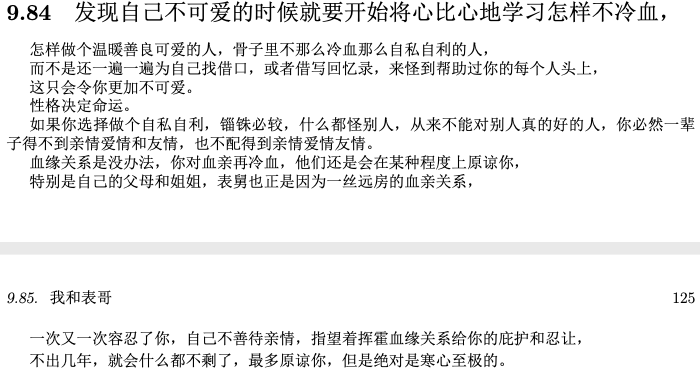
\includegraphics[width=.9\linewidth]{./pic/p1p125.png}
\end{center}

\begin{center}
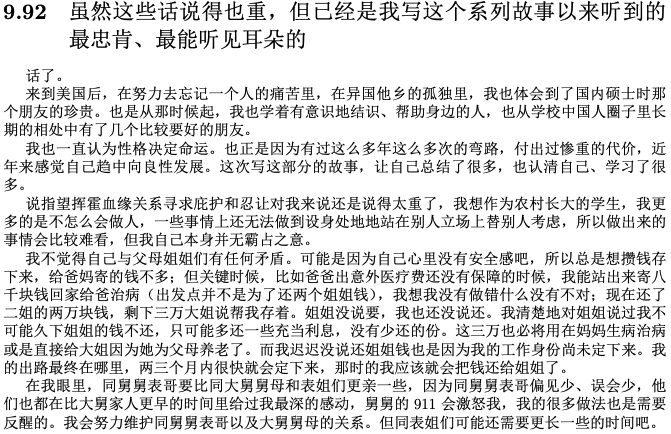
\includegraphics[width=.9\linewidth]{./pic/p1p128-3.png}
\end{center}

请你看到,每当我与表哥的关系亲密一点儿,比如12年春天,把自己的LinkedIn的名字改成与表哥神似,则大表姐会躲我躲到天边;
12年9月写出那份作业后,先前10、11年职场中作了三大的托儿的那个职场所谓的朋友也永远消失了
后来表姐与我的联系仍然是时断时续、全凭任凭三大支配,是为什么?

\subsection{push当事人从专业职场转向非专业职场洗脑贴}
\label{sec:org8724a44}

\begin{center}
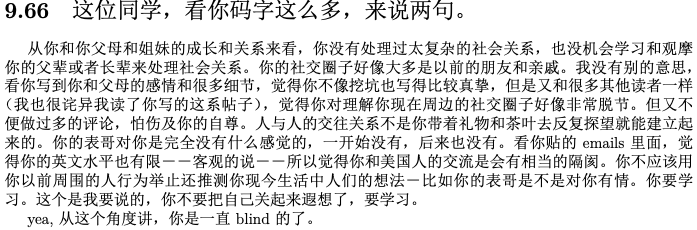
\includegraphics[width=.9\linewidth]{./pic/p1p115.png}
\end{center}

需要一个过渡:他们是如何炒作网红的?具体的炒作手法和手段有哪些?

结合后来表哥、舅舅的事实、史实来写

\subsection{混水摸鱼、混淆视听的搅水贴}
\label{sec:org2f3d9d3}

\begin{center}
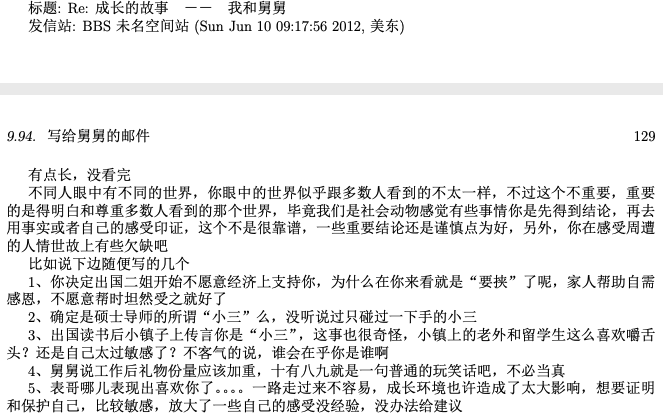
\includegraphics[width=.9\linewidth]{./pic/p1p129-2.png}
\end{center}

\section{我最亲爱的表哥(2):我要留在你身边!}
\label{sec:orgc4eb6eb}

\section{申请计算机的硕士:为什么我想读计算机,我的优势,我的起点、我的分析能力在哪里等等(可能会跳过这个)}
\label{sec:org1146ed0}

\section{读计算机专业时的必要大事记}
\label{sec:org88e4632}
\begin{itemize}
\item 本系大牛对于速读速毕业的转专业(大龄)学生的做法与认可度
\item 本系大牛对于推进广大学生朋友、国际留学生婚姻婚事的做法
\item 本系对于国际留学生专业方向的推向(把另一个大25岁马推到这里来)
\item 毕业时系里方面有劝过的读博士的可能性,如果我读博士,并说如果我不喜欢表哥,可以不用嫁给他
\item 我所杖着的自己如日中天的名气,疏不知,当日如日中天的名气也不过是日后折腾你人生的枷锁
\end{itemize}

\section{与警察冲突事件的原因与进展分析(这个应该可以不要了)}
\label{sec:org58b18cb}
\begin{itemize}
\item 2012年、2013年去找过表哥:为什么,结果怎样
\end{itemize}
\begin{center}
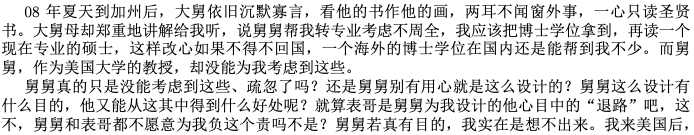
\includegraphics[width=.9\linewidth]{./pic/p1p136-5.png}
\end{center}
读博士与否:一个负责任的做法到底应该是怎样的呢?
\begin{center}
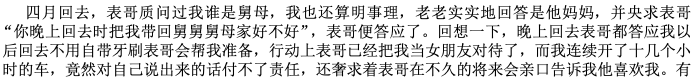
\includegraphics[width=.9\linewidth]{./pic/p1p125-3.png}
\end{center}
谁是舅母?
\begin{center}
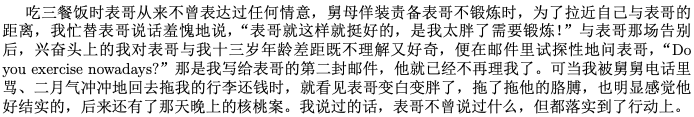
\includegraphics[width=.9\linewidth]{./pic/p1p125-2.png}
\end{center}
具体地去分析
\begin{center}
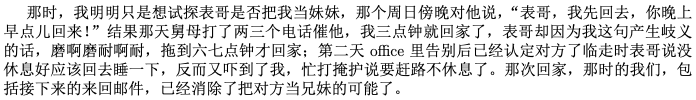
\includegraphics[width=.9\linewidth]{./pic/p1p125-1.png}
\end{center}
那时我幼稚的思维、长途开车后的疲累把智商都给彻底智熄了吗?当然不是。
\begin{center}
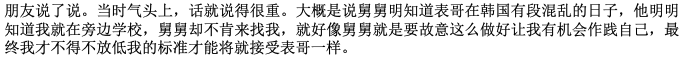
\includegraphics[width=.9\linewidth]{./pic/p1p49-3.png}
\end{center}
表哥在韩国有段混乱的日子,实则是我自己想出来的
\begin{center}
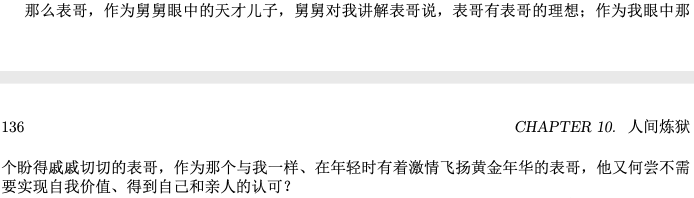
\includegraphics[width=.9\linewidth]{./pic/p1p135-05.png}
\end{center}
表哥的理想?

\section{2013 Summer Intern计算机专业的11周实习总结}
\label{sec:org268c6da}
\begin{itemize}
\item 把小导师当成记忆深处、理想里、脑海中、写给我的邮件里对我的职场工作有着清晰地表达、当年职场中意气风发的表哥,合二为一
\end{itemize}

\section{三大炒作网红、逼良为娼洗脑记(3):三大自导自演炒作出的自家网红的结局预告:专业职场的、非专业职场的将来被逼性奴 2014年7月}
\label{sec:orgbd60b7c}

  \begin{center}
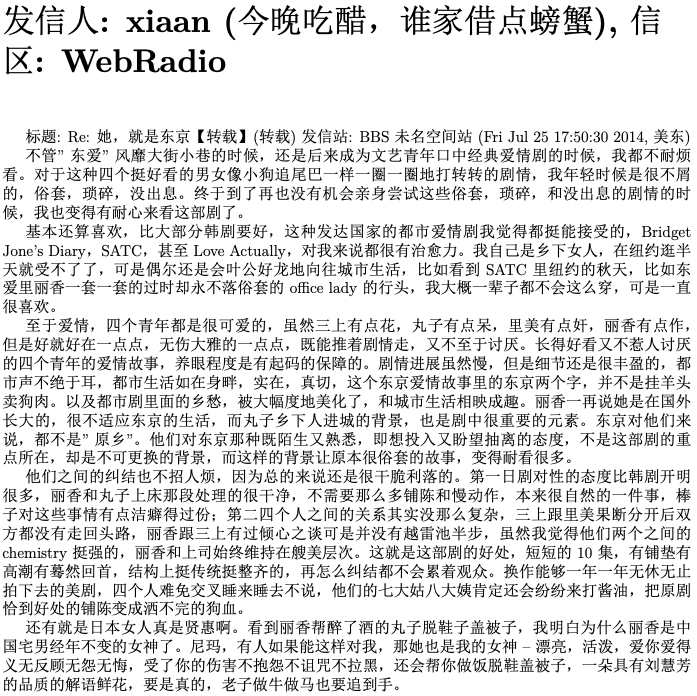
\includegraphics[width=.9\linewidth]{./pic/p2p201.png}
\end{center}
问号的争当版主,与大主力的转移;用《金瓶梅》给被逼当事人洗脑

\section{毕业后的去向:不想读博士的原因;不想黑下来;结婚:生病有生以来最严重的一场病,怕是会永远失去表哥了}
\label{sec:org71f3bc1}
  2015年来到加州,表姐逼我黑下来,不给我作经济担保,而我一定不要黑。(注意:三大网上炒作的舆论与自己现实生活中的差别与混入,对现实生活的影响)
不想读博士
去硅谷,读了三个学期
\begin{itemize}
\item 黑与不黑:在我内心深处的区别: 身份不敢黑: 怕会永远地失去表哥;又读了三个学期的软件工程
\end{itemize}
\section{结婚}
\label{sec:org0de0b2b}

\section{另一份专业相关的工作}
\label{sec:org36bcb94}
\begin{itemize}
\item 对于紧急事件的处理:被逼女生怀孕,三大黑势力的处理办法:用一份工作确保被逼当事人不会怀孕和生小孩
\item 三大的处理
\item 后续:相关部门工作人员来作报告
\item 我离职
\end{itemize}

\section{职场生涯(专业职场、非专业相关职场)中的性骚扰}
\label{sec:org0351d43}
\begin{itemize}
\item 补充2011年3月统计专业中职场性侵诽闻(2013年3月补充的我对那件事的个人认识)
\item 个人个性中对于界限的认定:个性中对男女有别等的界定与认知
\begin{itemize}
\item 2011年年底、2012年年初时朋友三青问那个小球、而后来再去那个餐厅吃饭时,我给他指当时我们坐在什么位置的那种潜意识里的模糊
\item 2013年三星实习时那个星期五,问A为什么昨天不能告诉我我的新项目是什么,对于IPO是否会给我OPT延期的这种清楚与潜意识里的不清醒: \textbf{若明若暗、似有似无的潜意识} 神合其神的潜意识:可以来个合集
\end{itemize}
\end{itemize}

\section{离职后的非专业相关硅谷生活,简略快结束}
\label{sec:org7b2cb32}
\begin{itemize}
\item 为三大周边产业(三大的托儿们的生意)圈钱,兼做忠诚度测试,并攻心
\end{itemize}

对于自己受这么多年苦累的心理不衡,2014年夏天我在San Jose Downtownn所租住的7房子是王夏华提前帮我找好的
\begin{itemize}
\item 要不要从王夏华处要结婚彩礼呢?求仁得仁,能够得到表哥我就很知足了。只求我不负任何人,就可以了
\end{itemize}
补细节:这次来写,可以清楚地看到我的情伤状态有所提升,这次写的过程中我也回忆起很多被我遗忘的细节(就像Eecs四个字母崩入我的脑海,很多记忆深处的东西往外崩,我想起来了很多的细节)
12年08年夏天舅舅把我送到加州硅谷人间繁华地来体验大城市的繁华。十多年里,我看透了城市繁华背后的虚幻、对大城市不再向往、没有留念、甚至想要离去远去避开它的喧嚣嘈杂。

我想要离去,我要去哪里呢?当然去表哥的城市去找表哥呀!

\begin{itemize}
\item 我喜欢大自然:厌倦了城市,我想回到农村去,回到像舅舅表哥所喜欢的可以轻松回归大自然的地方去!
\item 作为一个农村长大的孩子,我喜欢广袤的大自然,我喜欢雨过天晴的滋润清新,我喜欢雨后的青草味道;
\begin{itemize}
\item 小时候二姐带我们去叔叔家做客,我们一定会选择下雨天去,应该下雨天去叔叔用他的渔网打鱼会比较有渔获,而我就是那个喜欢跟着叔叔去广袤的大自然中去呼吸新鲜空气的、捡渔虾的小P孩;
\item 小时候同爸爸出去打鱼的时候夜晚里夜幕降临露水落下、滋润清新的夜幕下的青草味道;
\item 我喜欢大学时期武汉的梅雨季节的雨水,这些雨水滋养着我的灵魂(和12月7日的广场绘画展,艺术陶冶情操,我的心灵得到洗涤)
\item 2005年秋天当实验室一定不再是我的选择,我选择了去山青水秀的广西养病,帮助自己早日从困难中摆脱出来
\item 2013年夏天我终于鼓足勇气去锻炼身体,我把自己锻炼得比较好,我也把自己工作时的精神状态调整得比较好
\end{itemize}

我会求仁得仁,回到家乡,回到表哥所在的地方, 至于王夏华她们要不要报点儿恩,那是她们的事,我管好自己就可以了
另,不要急于毕业,推动博士生的培养,发扬我亲爱的表哥将博士读了8年的精神
硕士研究生考试成绩、生命是一场历程。我终于明白考硕士的315对于我来说,是给了我一次机会,同样的是UI的录取
以及与国内导师的感情戏、
与同学的朋友情
IPO 
不仅仅是舅舅带我到那繁华的硅谷逛了一圈,他们也通过努力把我带到异国他乡逛了一圈。受到过挫折,但这趟人生苦旅,深深地诱变了我,我为自己今生有机会变成如今拥有灵魂的这个样子感到骄傲、为自己今生能够拥有表哥的爱情感到无限满足和开心!
\end{itemize}

\section{我最亲爱的表哥(3)}
\label{sec:org3918592}

亲爱的表哥,写到这里,我终于是完成了我们共同完成的一件壮举:破除三大中文网站逼良为娼的产业化操作,将他们如此炒作自家网红、并最终逼良为娼的产业链彻底白菜化,让他们这一见不得光的暗箱操作彻底见光死、让他们的这个产业链在广大小市民、老百姓心目中了然于胸、一见便知、心知肚明,让越来越少的女性、女留学生们陷入到我曾经所遭遇的这些困境中来!

亲爱的表哥,这件事情、在你的发动、我的无限制配合下,我们终于是完成了一件壮举,我们做到了:为往事干杯,为我们自己干一杯!

到现在,我终于明白,09年秋天学期、舅舅不早不晚在我统计专业的最后一个学期、为我从韩国搬回来的表哥,就是真真正正要表哥作我的坚强后盾来着!不是早年间我那12年表哥亲手播打911后我自己反省出来的自已是寄生草寄生虫,舅舅帮我搬回来的就是真真正正、我内心里最想要的,我的矿世爱情和我今生的终身归属!

有一种感动惊心动魄,有一种遭遇万劫不复,当我们遭遇爱情、追寻过梦想、历经沧伤,当我们回归到梦开始的地方、回到我们出发的原点,亲爱的表哥,你还在等我吗?

亲爱的表哥,你可以接纳我吗?你是否也如我般曾经沧海(难为水)?你的沧海里是否可以容纳我的一滴眼泪?
\end{document}